%!TEX root = ../main.tex

\section*{Supplementary figures}

  \renewcommand{\thefigure}{S\arabic{figure}}
  \setcounter{figure}{0}

  \begin{figure}[h!]
    \centering
    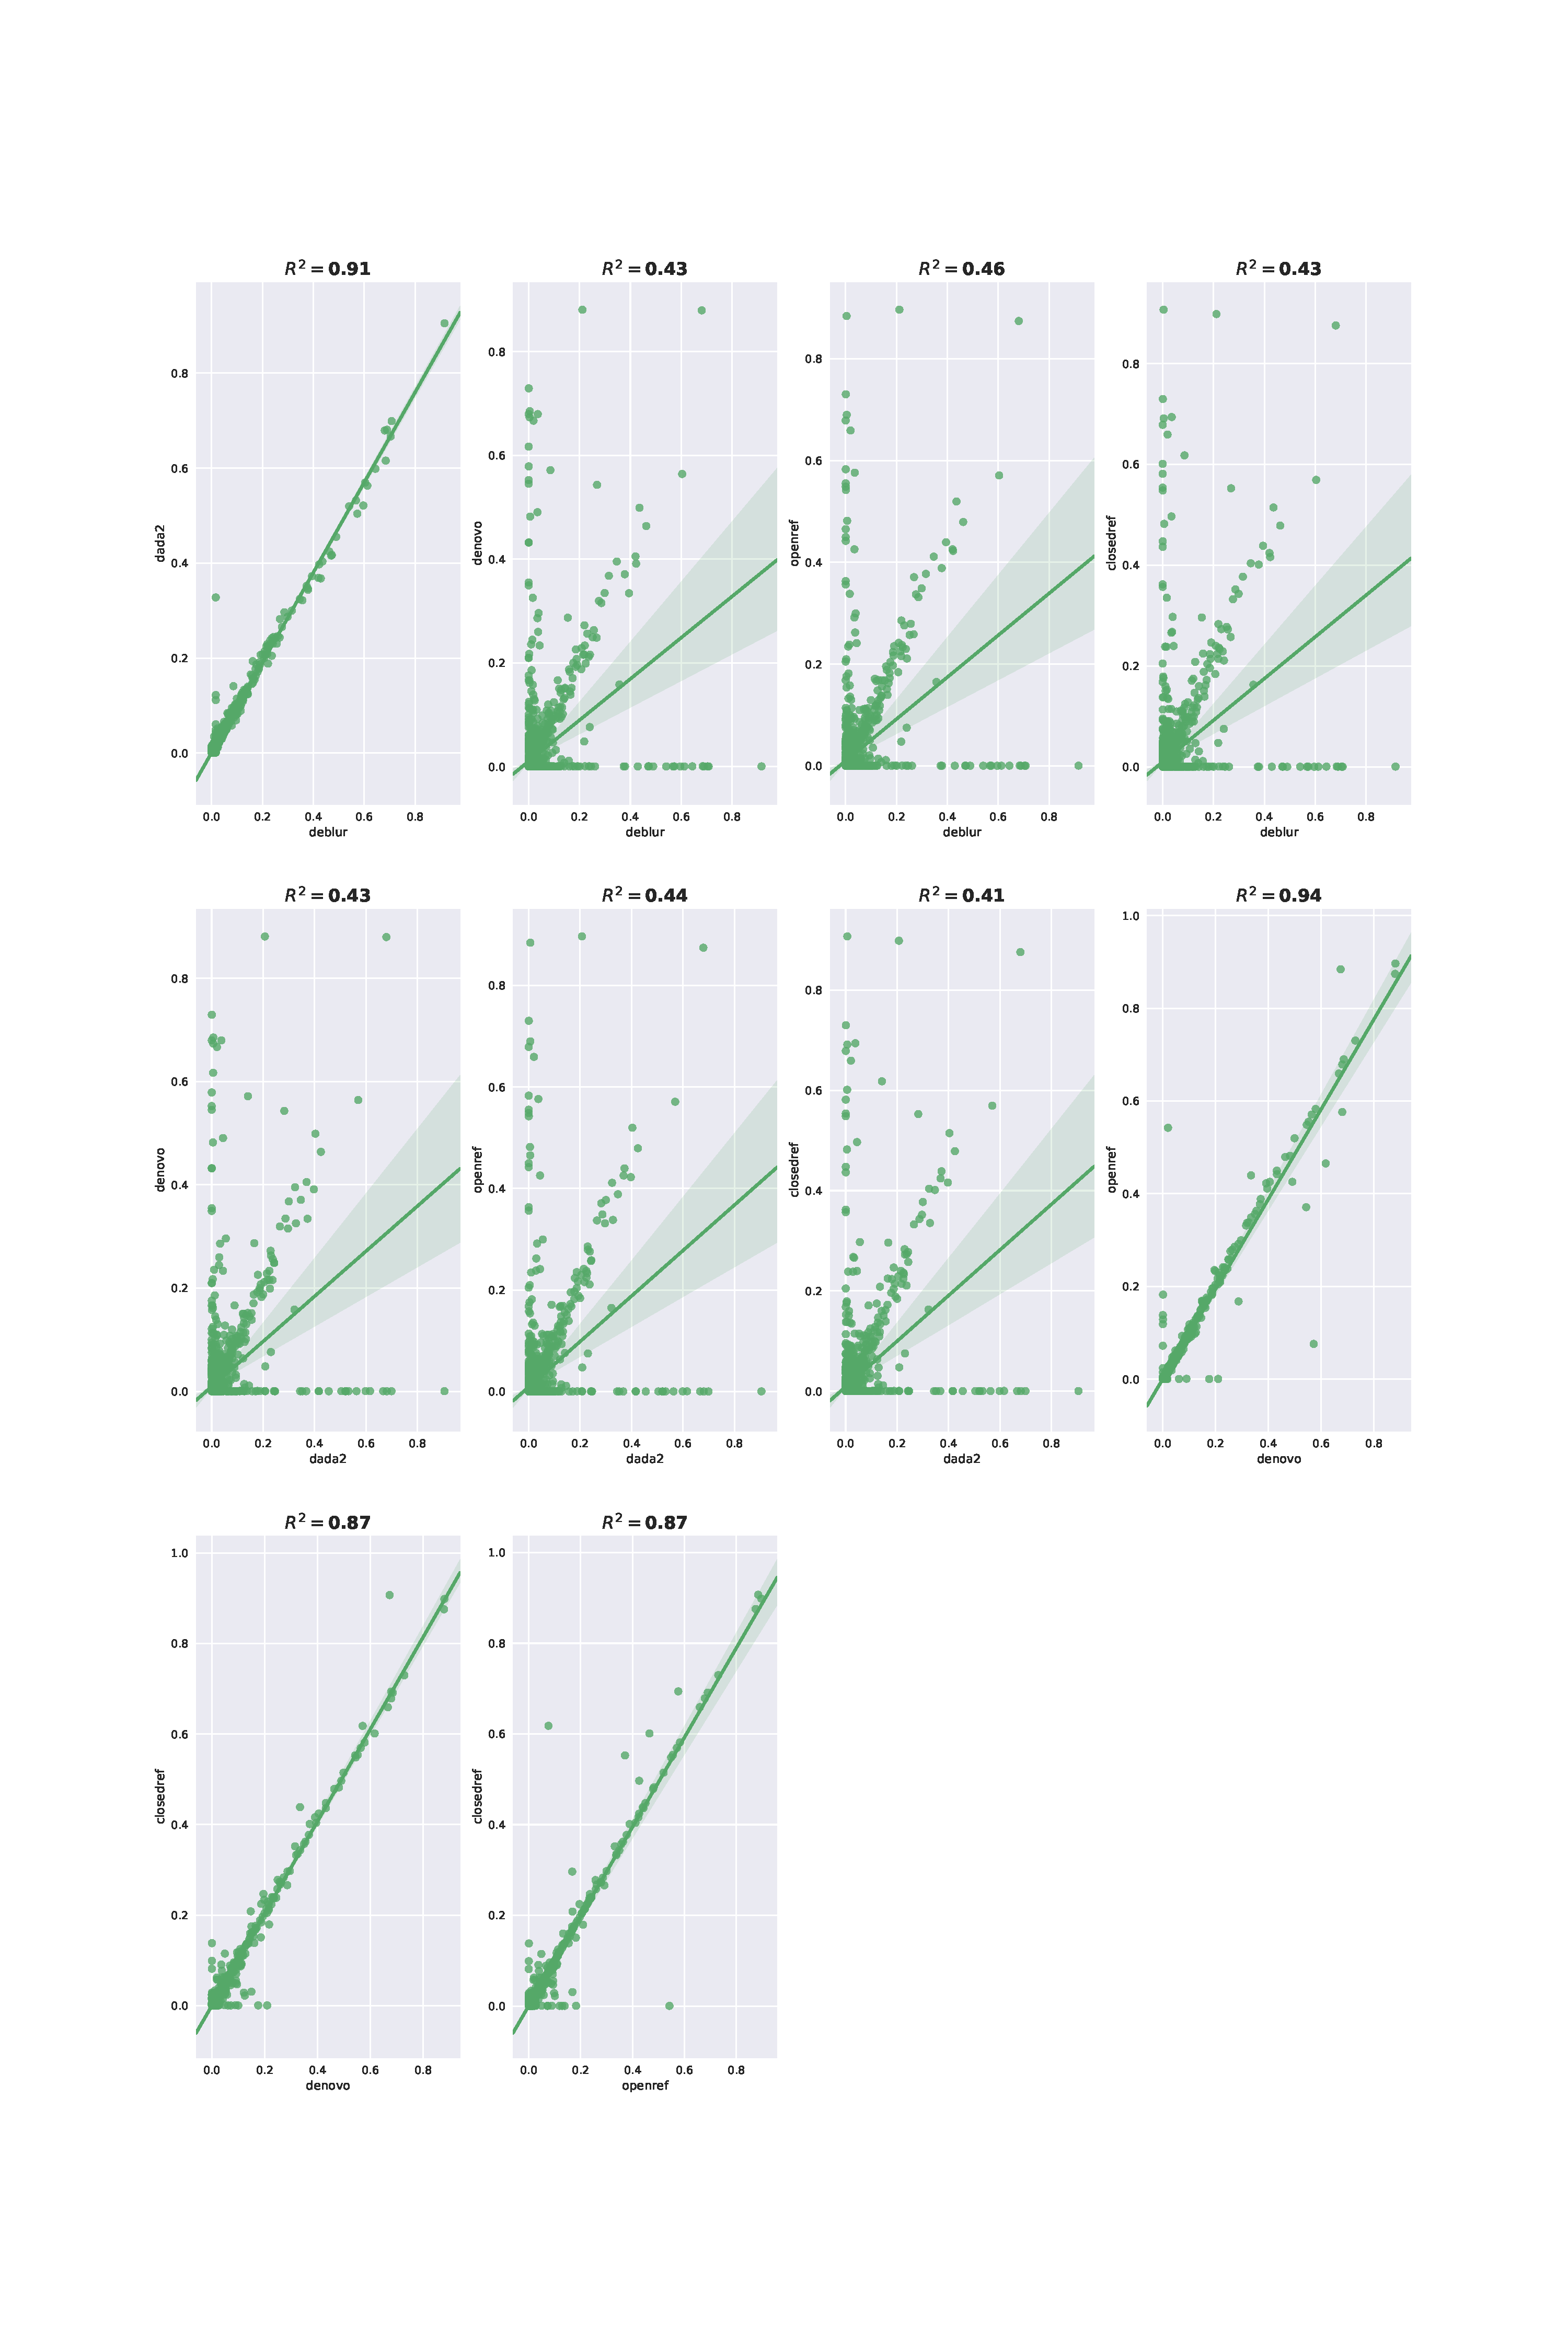
\includegraphics[width=0.93\textwidth]{all_denoise_reg.pdf}
    \caption{
      \textbf{Pairwise regression plots for all the denoising methods}.
    }
    \label{fig:all_denoise_reg}
  \end{figure}

  \begin{figure}[h!]
    \centering
    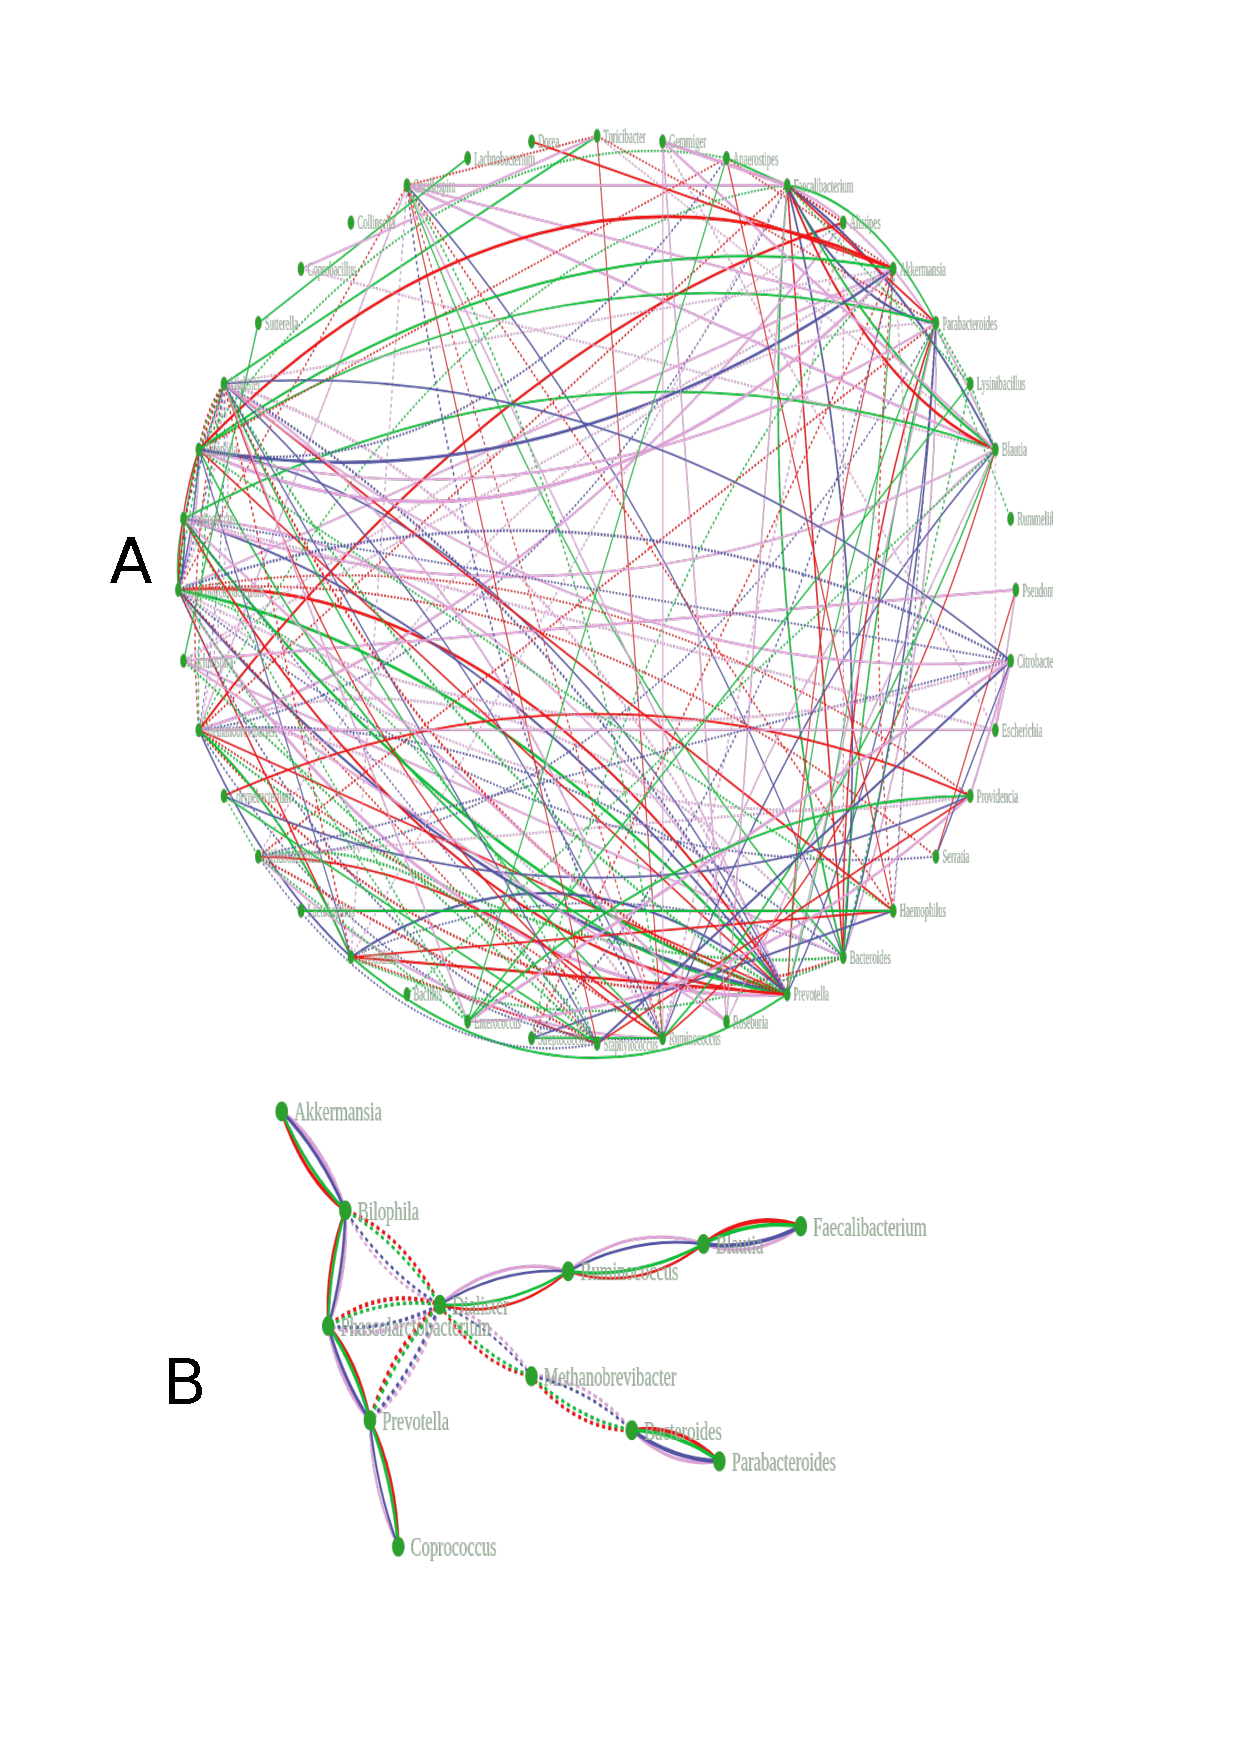
\includegraphics[width=.9\textwidth]{denoise_network.pdf}
    \caption{
      \textbf{Networks generated using various denoising methods.}
      The denoising methods used in this result are closed-reference clustering, open-reference clustering, denovo clustering and \ac{dada2}.
      The database (\ac{gg}) and network inference methods (\ac{sparcc}) were kept constant.
      (A) The set of interactions predicted by using all the methods (union)
      (B) The set of interactions that were common to all the methods (intersection)
    }
    \label{fig:denoise_network}
  \end{figure}


